

\documentclass{scrippsthesis}
%\documentclass[a4paper,11pt,twoside]{scrippsthesis}
%\usepackage[pass]{geometry}
%%% HEADER INFORMATION %%%

\title{Practical Chaos:  Using Dynamical Systems to Encrypt Audio and Visual Data}
\author{Julia Ruiter}
%\reader{Chris Towse}
%\reader{Adam Landsberg}

%%% Including new commands and packages.

% Allows for auto formatting of theorems,
% definitions etc.
\usepackage{amsthm}
\usepackage{graphics,graphicx}
\usepackage{tikz}
\usepackage{verbatimbox}
\usepackage{textgreek}
\usepackage[toc,page]{appendix}
\usepackage{float}
\usepackage{amsmath}


\newtheorem{thm}{Theorem}[chapter]
\newtheorem{lem}[thm]{Lemma}
\newtheorem{prop}[thm]{Proposition}
\newtheorem{cor}[thm]{Corollary}

\theoremstyle{definition}
\newtheorem{defn}[thm]{Definition}
\newtheorem{ex}[thm]{Example}

\theoremstyle{remark}
\newtheorem*{rmk}{Remark}
\newtheorem*{notn}{Notation}
\newtheorem*{pf}{Proof}

% Add any new commands here.
\newcommand{\Q}{\mathbb{Q}}
\newcommand{\Z}{\mathbb{Z}}
\newcommand{\F}{\mathbb{F}}
\newcommand{\R}{\mathbb{R}}
\newcommand{\NN}{\mathbb{N}}

%file path for images


%%%  END HEADER %%%

\begin{document}
%\begin{comment}

\frontmatter

\maketitle % Title page
%
%
%%%% ABSTRACT.
%
\begin{abstract} 
Although dynamical systems have a multitude of classical uses in physics and applied mathematics, new research in theoretical computer science shows that dynamical systems can also be used as a highly secure method of encrypting data.  Properties of Lorenz and similar systems of equations yield chaotic outputs that are good at masking the underlying data both physically and mathematically.  This paper aims to show how Lorenz systems may be used to encrypt text and image data, as well as provide a framework for how physical mechanisms may be built using these properties to transmit encrypted wave signals.
\end{abstract}

%%% CONTENTS, FIGURES, TABLES
\tableofcontents
\listoffigures
%\listoftables

%%% ACKNOWLEDGEMENTS.

%\begin{acknowledgments}
%...(write here later)
%\end{acknowledgments}

%%% End of the front matter.

%% MAIN MATTER - INCLUDE THE CHAPTERS.
\mainmatter

% CHAPTERS %

\chapter{Lorenz, Liu, and Other Chaotic Systems}

\par Thanks to $\it{Jurassic Park}$, most everyone is familiar with the idea of the ``Butterfly Effect'':  the idea that one small perturbation in the present can set the future on a wildly different course.  This idea comes from Ed Lorenz, chaos theory's pioneer, and his observations of dynamical systems with strange attractors, that is, systems of equations that have an element of chaos built into them.  These systems are a part of the family of Lorenz equations and are of the following form:
%
\begin{equation}
\begin{cases} 
\dot{x} = \sigma(y-x) \\ 
\dot{y} = rx - y - xz \\ 
\dot{z} = xy - bz
\end{cases}
\end{equation}
%
%Figure \ref{fig:genLorenz} original Lorenz system
%  use math mosde $_$ for all variables in paragraphs
where the dot denotes the first time derivative of each variable, and with the Prandtl number ($\sigma$), Rayleigh number($r$), and $b$ all greater than 0.  The aperiodic nature of this system defined by a total lack of fixed points and quasiperiodic orbits for any initial trajectory means that the outcome is very sensitive to its initial conditions.  The deterministic nature of the system, the fact that its irregularity comes not from randomness, but the nonlinear relationships of variables, means that once the initial conditions have been set, the outcome at any given time $t_0$ is always going to give the same values $x$, $y$, $z$.  These two attributes make the Lorenz equations a very good candidate for an encryption system (more on that in the next chapter).  

\begin{figure}[H]
    \centering
	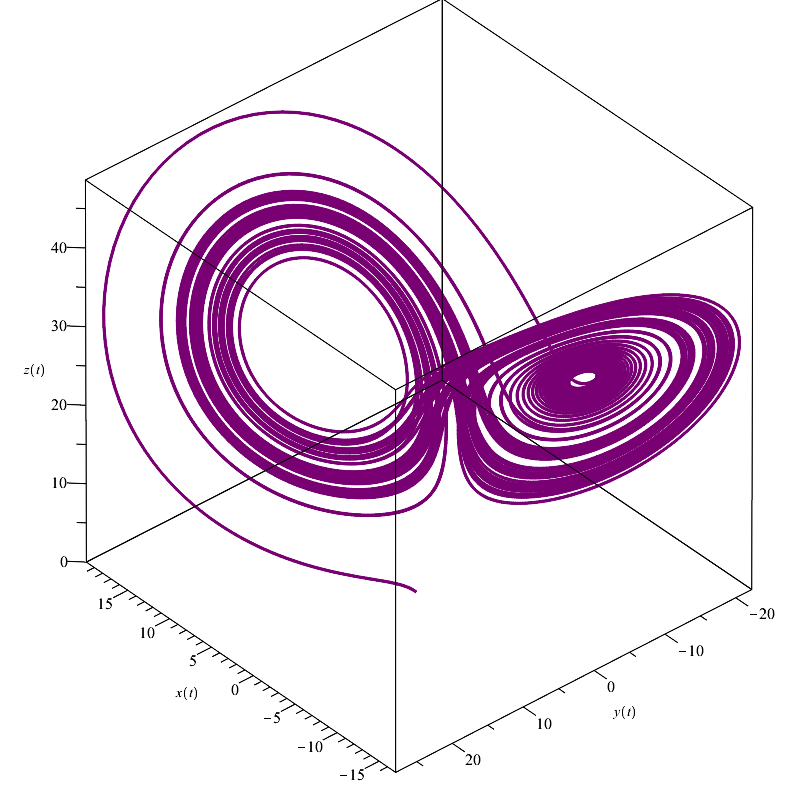
\includegraphics[width=\linewidth]{lorenz2.PNG}
	\caption{Lorenz System where $r = 28, \sigma = 10, and b = 8/3$. *}
	\label{fig:genLorenz}
\end{figure}

\par In other words, chaotic systems have a dense orbit, meaning that the system has at least two orbits that are sensitive to the initial conditions, thus excluding systems with only one cycle as well as systems consisting of just an equilibrium point which are systems with clear orbits in their phase space (to be defined in glossary). 

\par The most notable feature of the Lorenz systems is that it contains a strange attractor.  An attractor is a subset A of the system's phase space where the neighborhood of A is defined as being the basin of attraction, the basin of attraction being the region of phase space where the system starts to show cyclic action, usually resulting in a stable orbit, or condensing towards a point.  Strange attractor differ, however, in that given any two points arbitrarily close to each other in one orbit, several orbits later will be arbitrarily further away, rather than same or closer.  It is this quality that makes the system chaotic.

\par What is important to note, though, is that not all values of $r$, $b$, and $\sigma$ will yield a chaotic system. An analysis of the bifurcation diagrams (a diagram that shows values for which there are stable and unstable equillibria) of $r$ help explain why only certain values work.

\par for Lorenz systems, there is always an equilibrium at the origin $(0,0,0)$, this is true of any variation of the Lorenz system, using any values $b$, $r$, and $\sigma$.  However, if $r>1$, then other critical points appear:
%
\begin{equation}
(\sqrt{b(r-1)},\sqrt{b(p-1)},(r-1))
\end{equation}
\begin{equation}
(-\sqrt{b(r-1)},-\sqrt{b(p-1)},(r-1))
\end{equation}
%
which means the system exhibit cyclical behaviour if and only if $r$ and $\sigma$ are positive and have the property that:
%
\begin{equation}
\sigma > b + 1 
\end{equation}
\begin{equation}
r > \sigma \frac{\sigma + b + 3}{\sigma - b - 1}
\end{equation}
%
because of that, the original version of the Lorenz system (and the one used later in this text) is usually restricted to values close to:
\begin{equation}
\begin{cases} 
r = 28 \\ 
b = \frac{8}{3} \\ 
\sigma = 10
\end{cases}
\end{equation}
%
which are the original set of values that Lorenz accidentally discovered that exhibited chaotic behaviour.

\par What happens if the variables don't all fall in this range?  Take this example where only the value of \textsigma has been altered:
%
\begin{figure}[H]
    \centering
	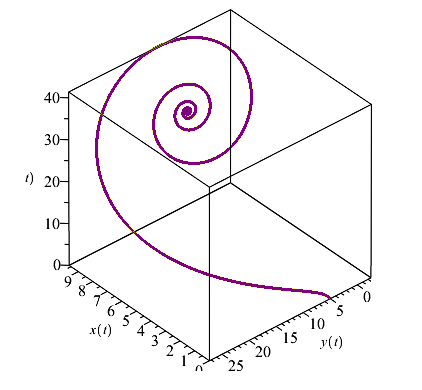
\includegraphics[width=\linewidth]{lorenz_s2.png}
	\caption{Lorenz System where $r = 28, \sigma = 1, and b = 8/3$}
	\label{fig:badLorenz}
\end{figure}
%Figure \ref{fig:badLorenz} nonchaotic Lorenz system
%
As you can see, the resulting graph is not at all chaotic, with x, y, and z all having a fixed limit (regular attractor) as time goes to infinity, or otherwise exhibiting standard actions as dynamical system.  This means that distance between two points at t0 will always be larger than the distance between those points at a later $t_1$, meaning that it is easy to predict how the system behaves over time.  Because of the predictability, a Lorenz system with these parameters cannot be used to encrypt information, as values follow a predictable pattern.  For that reason, we will only consider Lorenz systems with chaotic action (like those mentioned at the beginning of the chapter) as candidates for strong encryption.

%
\subsection{Liu and Chen Systems}

\par Lorenz systems are not the only type of dynamical system that exhibit this sort of chaotic behaviour.  Two other systems, Liu and Chen, are variations of the Lorenz system, with slightly different dependencies and thus different usable chaotic parameters.

\par Although it is a bit difficult to see, the Chen and Liu systems actually shows greater levels of chaos that the Lorenz system, and thus are better candidates for chaotic encryption.  Because of this, these systems, though only discovered in the past 15 years,  are most often used and referenced in current publications in this field.

\par Take the Chen system:
%
\begin{equation}
\begin{cases} 
\dot{x} = a(y - x) \\ 
\dot{y} = (c - a)x + cy + xz \\
\dot{z} = xy - bz
\end{cases}
\end{equation}
%
which is chaotic for values close to $\{a,b,c\} = \{35,3,28\}$ (note, the last parameter is the same as that of the Lorenz system since the path of z is still depended on the same interaction of x and y).  The Chen system is more volatile in its changes in x and y than the Lorenz system, meaning there is a larger variability in what $\{x,y,z\}$ values are output at any adjacent values t, thus making the system harder to predict.

\begin{figure}[H]
    \centering
	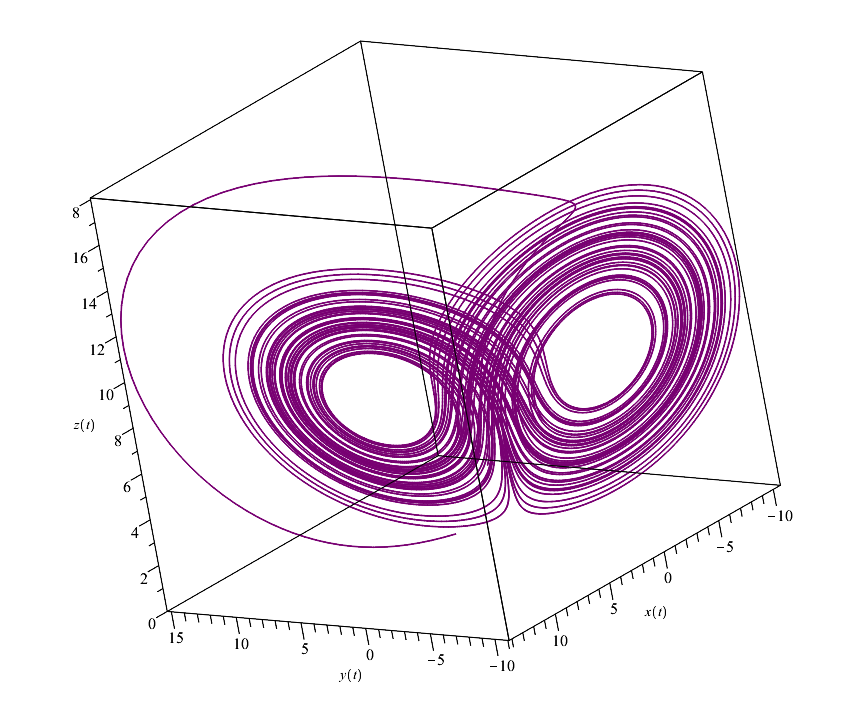
\includegraphics[width=\linewidth]{chen2.PNG}
	\caption{Chen system}
	\label{fig:chen}
\end{figure}
%Figure \ref{fig:chen} general Chen system

\par Now take the Liu system:
%
\begin{equation}
\begin{cases} 
\dot{x} = a(y - x) \\ 
\dot{y} = bx - kxz \\
\dot{z} = hx^2 - cz
\end{cases}
\end{equation}
%
\begin{figure}[h!]
	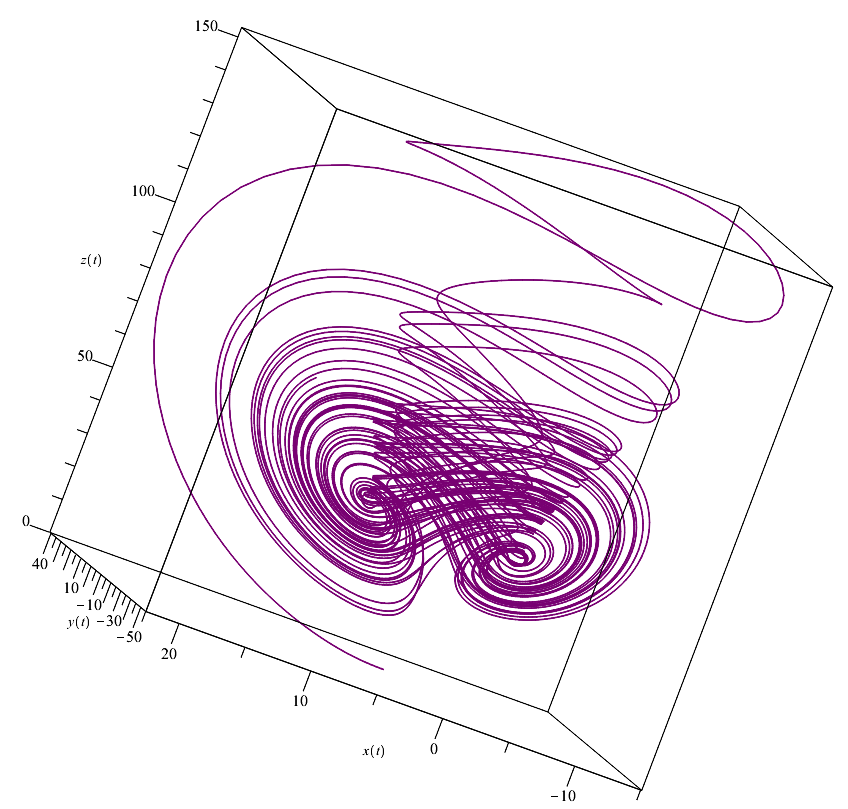
\includegraphics[width=\linewidth]{liu2.PNG}
	\caption{Liu system}
	\label{fig:liu}
\end{figure}
Figure \ref{fig:liu} general Liu system
%
which is chaotic for values close to $\{a,b,c,k,h\} = \{10,40,2.5,1,4\}$.  This system is not only more chaotic (thanks to the x squared term in the z-partial), but because it has so many more fixed parameters than the other systems, is even harder to decrypt.  And because of the nature of chaotic systems, even being 0.00000001 off from any one initial condition can drastically change the output values.

Although these two systems, like the original Lorenz system, can only create chaotic outputs given a narrow range of constant parameters, again,but because the systems are continuous, there are infinite possible starting inputs that yield vastly different "butterfly graphs.  This sensitivity will become important in the next chapter when we talk about cryptographic applications of Lorenz and Lorenz-like systems.

\par 

%


%\end{equation}
% backslash square bracket to start equation
% \cite to cite in text
% tex will not display sources that are not refrenced
% tex is stubborn, will not allow you to tell it where to put figures

\chapter{Cryptography}

At the core of cryptography is one premise:  Alice wants to send a message to Bob, but is afraid of Eve intercepting and reading it.  Alice has no control over whether or not Eve will or won't get ahold of her correspondences, but she is able to control how easy it is for Eve to interpret and thus understand the content of the message.  However, Bob still needs to be able to decypher the contents of the message that is being sent to him, so Alice must come up with some sort of reversible system that will mask her message; a method that successfully allows for both of these criteria is called a \textit{cryptosystem}.

Cryptosystems can range from the familiar Caesar Cyphers from passing notes in elementary school to complex numerical systems only solvable by computers.  A good cryptosystem is one that is very difficult, or even impossible, to decrypt unless you have a particular set of information known as a \textit{key}.  The difficulty of encoding, or encrypting, the message is irrelevant to the strength of the cryptosystem, but certainly the easier it is to encrypt, the more useful of a system it is.  In order to explain how exactly  Liu, Chen, or Lorenz equations make a foundation for a reliable cryptosystem, I will compare it to a simpler system, then explain the particular advantages of \textit{Chaotic encryption} over other methods.

\subsection{Choosing a Key}

"Buj'i we rqsa je jxu Squiqh Sofxuh unqcfbu", or rather, "Let's go back to the Caesar Cypher example". 

A cryptosystem's key is the transform from the original message to the encrypted one.  In this case, it's clear that there's a one for one substitution for each character and, in particular, that shift is 16 letters to the right; therefore the key is 16. All Bob has to do to read Alice's message is use the key in some sort of function in order to invert the decryption; so here, shift 16 characters to the left.  Remember, a good cryptosystem is largely dependent on choosing good keys.  It is obvious that there are only 26 possible keys to choose from, and setting the key equal to 26 is a very poor decision.  Even 13 is a bad idea since it is a common key used for Caesar Cyphers and Eve would likely figure out that key quickly.  If Eve figures out the key, or manages to find some other method of breaking the system (say, by using a code breaker she finds online), then the system is compromised and no longer a secure means of communication.

We can extend this idea to other cryptosystems--every encryption method will have its trivial keys, redundant keys (for the above example, a key of 42 would yield the same result, as would -10), and keys that simply just don't work (how on Earth would you shift 1.75 letters to the right?!).  However, it is not always easy to tell if a chosen key will work.  One might think that any values ($a, b, and r$) can work in the differential equations, but because of the nature of \textit{Strange Attractors} inherent to these types of graphs, that's not always the case.  As we saw in the previous chapter, some values yield a predictable graph,  meaning that Eve could use the encrypted message to fairly easily create a model and break the code.  

Other values may yield other strange results, like cyclic outputs.  If you were to draw a steady state diagram of these degenerate systems, you would see cycles in the graphs, meaning that two different input values can encrypt to the same value, and Bob wouldn't know which output is correct, if he even realizes the redundancy at all.  So while it is certain that there are infinite values of ($a, b, and r$) that will produce chaotic output and therefore make good keys, it is nice to know that there is a smaller subset of that infinity that are easy to find as well as \textit{guaranteeing} non-degeneracy.  These keys ensure a secure system because, unless Alice and Bob agree on a trivial key (say, some nice round number close to the base Lorenz parameters), it would be near impossible for Eve to brute force break the system by trying every possible key because there are infinitely many of them.

\subsection{Creating an Encryption System}

Every cryptosystem has three components: ($c$)--the encrypted message, ($k$)--the key, and ($h$)--the function the transform ($c$) back to the original message ($m$).  In the earlier example, each element of ($c$) had a 1:1 correspondence to an element of ($m$), and this is true for nearly all cryptosystems, for ease of encoding and decoding, particularly on the recipient's end.  Ideally, rather than have to solve each element individually (as one might do in a symbol substitution cypher), you will have a function ($h$) that will either directly give you the decoded message, or at least make it faster to decode each ensuing component of the message after the first.  Generally for any cryptosystem, these components will be defined by the functions:
%
\begin{equation}
    c = e ( m , k ) \\
\end{equation}
\begin{equation}
    m = h ( c ) \\
\end{equation}
\begin{equation}
    c \neq m   
\end{equation}
%
where ($h$) can be one or many functions in a system that decrypts ($c$) and where ($e$) is the function that encodes ($m$), but is not necessarily the inverse function of ($h$), particularly when ($h$) is a system of functions.  It is also important to note that a cryptosystem may have multiple keys, or each party may have their own personal key that the other party may not know.  ($h$) is determined by the type of system; all Lorentz systems have the same structure, where ($h(c)$) is simply the set of differential equations and k the constant scalars ($a, b, r, c, k$).  Generally, Alice will compute ($c$) and send it to Bob, who by prior arrangement knows ($k$) and therefore can decode the message using ($h$) and any other helper equations necessary.

How, exactly, ($c$) is transmitted is more flexible than with other cryptosystems.  Typically, encoded messages would just be sent in written form or typed, and is then just a numbers game on the other side.  However, physical chaotic systems also have the unique property in that they can synchronise with other systems, and therefore automatically decode if set to the same initial parameters, k.  This flexibility is what makes for a promising future in audiovisual encryption.









\chapter{Visual Static:  Using Dynamical Systems to Encrypt Photographs }

In order to truly scramble the contents of an image, you must not only transform the color values of each pixel, but also randomize the location of each pixel in such a way that both sets of data minimize loss in the encoding/decoding process.  Most encryption systems can only do the former, which is not sufficient for privacy since a lot of nearby pixels will be nearly the same color.  Having almost the same RBG/BW values, these nearby pixels will transform to relatively nearby values in the encrypted state.  This is not secure for two reasons:  1) a mapping of these values back onto a grid will still show the general outlines/contrast color locations as the original photo, and 2) knowing how close the transforms are to each other, one could use this to approximate the derivative values--which \textit{are} the Lorenz transform equations, thus allowing anyone intercepting the image to possibly reconstruct it, and much easier with non-chaotic transform equations.

It is the element of chaos in Lorenz systems that allows for a truly unpredictable shuffling pattern, thus making image encryption more secure than ever before.  One method of combining these two ideas into one cryptosystem has been proposed by a group of computer engineering in Istanbul.  In this section, I will outline the method, as well as discuss ways in which this cryptosystem may be simplified.

\subsection{Proposed Image Encryption System}

Two non-Lorenz chaotic systems run in tandem: 
\begin{equation}
    f ( p ) := p_{i+1} = \lambda_{1} * p_{i} ( 1 - p_{i} )
\end{equation}
\begin{equation}
    g ( p ) := p_{i+1} = \lambda_{2} * p_{i} ( 1 - p_{i} )
\end{equation}
one to encrypt the pixel color values denoted by ($f(p)$), and the other the pixel locations which we'll denote with ($g(p)$).  In order to minimize number of keys needed, the researchers use the two variable bifurcation equations to make the transformation, rather than have the variables depend on each other as in Lorenz-like systems.  This makes sense since they took care to make sure the two encryption systems use different \textlambda values. Since there are a finite number of pixel color values (256 each for red, blue, green, and brightness), and there are a finite number of pixels in the image, all ($x_{i+1}$) and ($y_{i+1}$) values are discrete and greater than or equal to zero.  This means that there are a discrete number of outputs to both ($g(p)$) and ($f(p)$).  The outputs for ($f(p)$) and ($g(p)$) need to be set to discrete values in order to make a new image.  This is done by taking a step down function, then taking ($f(p)$) modulo 256 and ($g(p)$) modulo the number of pixels in the image.  Finally, the outputs of these functions for each pixel are paired together, then reordered in ascending order based on ($g(p)$).  

\subsection{Possible Improvements}

It may seem that due to the chaotic nature of the transform equation, it should not be necessary to have two separate lambda values, especially since the outputs will be on different scales anyway sue to the different modulo values.  However, this is not enough, as nearby pixels have nearby color values and therefore nearby transformations.  If the same lambda is applied to both parameters, the new transform locations will also be nearby, and nearly the same color.  However, this can be solved by using a different type of chaotic equation; the Liu system we looked at back in Chapter 1 shows that nearby small values oscillate, and oscillate in unpredictable patterns.  If a large enough lambda is chosen, the nearby pixels will be less correlated to each other due to higher variation in derivative, and thus it is far more likely for other pixels from other parts of the image to end up nearby as well.

\subsection{Plotting Bifurcation Diagrams in Python}

This is the base Python code I used to plot the bifurcation diagrams of the various chaotic systems trying to understand where Yavuz, et. al got their "seed values", or ($r$) key values for the transformation.  The publication was vague on the exact numbers used, but after some trial and error, it became clear that any value of lambda would work, as long as the ($x_i$) and ($y_i$) values are discrete, which they are since they respond to pixel location and color values, with the lambda determining how chaotic the resulting system is (the more bifurcations present, the more chaotic the system).  This code is based on an open source GitHub repository owned by "Alain1405" which uses a numerical approach to solve differential equations.  Simply replace the return line in "def logisticeq(r,x)" with your 2 parameter differential, and adjust the plot limits if needed.

%\begin{equation}
\begin{lstlisting}
\begin{verbatim}

import numpy as np
import matplotlib.pyplot as plt


# Logistic function implementation
def logisticeq(r,x):
    return r*x*(1-x)

# Iterate the function for a given r
def logistic_equation_orbit(seed, r, n_iter, n_skip=0):
    X_t=[]
    T=[]
    t=0
    x = seed;
    # Iterate the logistic equation, printing only if  \
        n_skip steps have been skipped
    for i in range(n_iter + n_skip):
        if i >= n_skip:
            X_t.append(x)
            T.append(t)
            t+=1
        x = logisticeq(r,x);
    # Configure and decorate the plot
    plt.plot(T, X_t)
    plt.ylim(0, 1)
    plt.xlim(0, T[-1])
    plt.xlabel('Time t')
    plt.ylabel('X_t')
    plt.show()

# logistic_equation_orbit(0.1, 3.05, 100)

# Create the bifurcation diagram
def bifurcation_diagram(seed, n_skip, n_iter, step=0.0001,  \ 
        r_min=0):
    # Array of r values, the x axis of the bifurcation plot
    R = []
    # Array of x_t values, the y axis of the bifurcation plot
    X = []
    
    # Create the r values to loop. For each r value we will   \ 
        plot n_iter points
    r_range = np.linspace(r_min, 4, int(1/step))

    for r in r_range:
        x = seed;
        # For each r, iterate the logistic function and  \  
            collect datapoint if n_skip iterations have occurred
        for i in range(n_iter+n_skip+1):
            if i >= n_skip:
                R.append(r)
                X.append(x)
                
            x = logisticeq(r,x);
    # Plot the data    
    plt.plot(R, X, ls='', marker=',')
    plt.ylim(0, 1)
    plt.xlim(r_min, 4)
    plt.xlabel('r')
    plt.ylabel('X')
    plt.show()

bifurcation_diagram(0.2, 100, 5)
\end{verbatim}
\end{lstlisting}


\chapter{Synchronised Chaos:  Using Dynamical Systems to Encrypt Sound}

One advantage chaotic encryption has over other methods is that it can encrypt all kinds of data, from text, to images, to even sound. For sound, it is possible to have coupled chaotic systems--two or more remote oscillators that exhibit the same relationships in patterns of motion, allowing for secure communication over large distances.  This coupling property was originally theorized in 1989 by Pecora and Carroll based off of nonlinear spin wave properties in magnetic materials.  Systems can be synchronised by transmitting waves from the "master" system to the receiver system(s), although inexplicable, the more systems were coupled, the greater the lag time in oscillations between units.  It is important to note that the units to not have the exact same motion, but rather that their range of motion is proportionally similar in terms of components. 

However, the audio encryption done using the Pecora-Carroll method differs from the previous chaotic encryption methods mentioned.  While earlier systems used Lorenz equations as a transformation function to receiver, this method uses the chaos as a shielding "drone" under the transmitted message.  Rather, the message itself isn't encoded, but it is like a cryptosystem in that it requires the other party to know the parameters.  Here, the Lorenz system itself is the key--it tells Bob what to "noise" to filter out of the transmitted message c.


\subsection{Master-Receiver Setup}

There are two different setups for a synchronised chaotic system that allow for this sort of encryption that just vary in how the receiver unit interacts with the master.  While the transmitting unit (Alice's) has components in three directions, the receiving unit  is only going to have two directions giving output to Bob; the third direction is known as the \textit{driver}.  The driver parameter is what causes the resonance between the units, allowing for this communication between them.  Without loss of generality, let us assume the the driving parameter is ($x$).  This means that the receiving unit will not have an ($x_{r}$) equation, and that the ($y_{r}$) and ($z_{r}$) equations will only depend on the ($x$) signal being transmitted and the responses of each other.


The master can be set up to use the Lorenz system of encryption we are already familiar with:
\begin{equation}
\begin{cases} 
\dot{x_{m}} = \sigma(y-x) \\ 
\dot{y_{m}} = rx - y - xz \\ 
\dot{z_{m}} = xy - bz
\end{cases}
\end{equation}
which means that the receiving unit has the remaining equations, also in the form of the Lorenz system:
\begin{equation}
\begin{cases} 
\dot{y_{r}} = rx - y_{r} - xz_{r} \\ 
\dot{z_{r}} = xy_{r} - bz_{r}
\end{cases}
\end{equation}

However, there is a different chaotic system known as the R\"{o}ssler system that works, too. The master unit emits:
\begin{equation}
\begin{cases} 
\dot{x_{m}} = -(y-x) \\ 
\dot{y_{m}} = x - ay  \\ 
\dot{z_{m}} = b+z(x-c)
\end{cases}
\end{equation}
which leaves the receiving unit with the parameters: 
\begin{equation}
\begin{cases} 
\dot{y_{r}} = x - ay_{r} \\ 
\dot{z_{r}} = b+z_{r}(x-c)
\end{cases}
\end{equation}

Interestingly, since the coupled R\"{o}ssler system has less "keys", there is a more direct relationship between the {$y_{m}$} and {$y_{r}$} as well as the {$z_{m}$} and {$z_{r}$} units, meaning that the received and "decoded" message is more like the original than if passed through a coupled Lorenz system.  As desired before in the cases of image encryption, minimizing loss in the transmitted message is equally as important as the security of the system itself.  And although the coupled unit system has less keys, it is perhaps more secure than other cryptosystems because you need to have the coupled unit itself to decode messages, and if messages are transmitted real time, there is a minuscule chance of interception, rather than on an encrypted image shared over a computer. 

Most fascinating, though, is the fact that the receiving unit does not need to be running the same type of encryption in order to communicate with the master unit.  Hernandez et. al discovered that Lorenz systems could communicate almost equally as well with systems running Lu or Chen dynamical systems because all three sets of equations have the same ($\dot{x}$) dependence as each other.  When you make this parameter the driving parameter between the two units, it does not matter what the rest of the system is--the other parameters of the receiving system, as in the two cases above, are just responses to the driver.  However, as the other parameter relationships are different, a lot of noise remains in the decrypted message, so it is far from perfect.

\subsection{Is it Secure Enough?}

The mis-paired systems mentioned above to indicate that there could be a security risk inherent in coupled chaotic systems.  If it is possible for two dissimilar systems to yield similar success in decryption, is it then not possible for there to exist some other dynamical system that takes components of other systems and use it as a brute force break on a transmission?  For audio, perhaps, but image and text encryptions have far less data points, so the noise obscures a lot more, meaning that a brute force attempt like this is unlikely to get anywhere.






%\input{PhysApps}

\chapter{Goals and Future Work}

\subsection{Goals for Thesis}

\begin{enumerate}
	\item Describe the basics cryptography 
	\item Describe the nature of dynamical systems and chaos
	\item Describe the different types of chaotic encryption and how the key parameters vary
	\item Propose improvements for existing chaotic cryptosystems
\end{enumerate}

\subsection{Future Work}

I first became interested in chaotic encryption when I stumbled across a side-note in \textit{Nonlinear Dynamics and Chaos} by Steven Strogatz describing how one of his students had build a physical circuit that used the principles of chaos to encrypt then decrypt input signals.  Before I had a chance to tinker with circuits myself, though, I got sidetracked in all of the other applications of chaos, namely how its an emerging field of encryption, largely of interest to computer science researchers.  For further studies, though, I'd like to take the ideas and methods documented in this thesis and apply them to physical objects, such as building synchronised systems in a laboratory.  There is still a lot of be researched in making these physical systems more efficient and more easily adjustable to new keys and parameters.  I am also interested in testing these systems in various environments--does natural interference get filtered out in the encryption process, or can it obstruct decryption entirely?

%\end{comment}


%%% End of the main matter.
\backmatter

%%%% BIBLIOGRAPHY (Be sure cto compile with BibTeX to make this work!)
%
\nocite{*} % Show everything in bib file, not just things that are explicitly cited.
\bibliography{bibliography}
\bibliographystyle{alpha}
%\printbibliography


\end{document}

% double check/cross with original doc--might be undoing what is going on in 
% have to bibtex bibliography first, then can tex rest of file